%11/09 - Patricia Álvarez
\chapter{Alineamiento de secuencias}
Decidir qué caracteres investigar, y cómo codificarlos, es un primer paso crucial en cualquier análisis filogenético. 

\section{Tipos de caracteres}
Hay \textbf{sitios invariables} que no cambian en los distintos taxones. También hay \textbf{sitios filogenéticamente neutrales} que son autapomorfías. Los \textbf{sitios filogenéticamente informativos} son comunes por pares, por lo que son sinapomorfías. 

\begin{figure}[htbp]
\centering
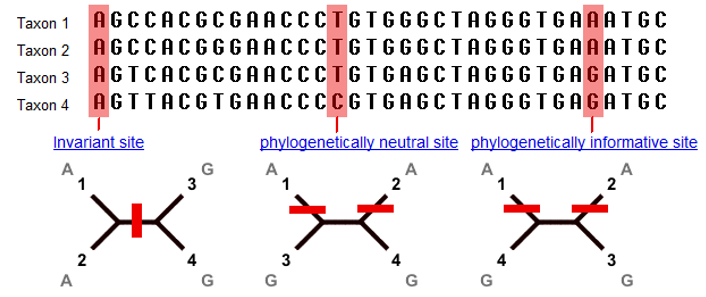
\includegraphics[width=0.5\linewidth]{figs/sitios-informativos.png}
\caption{Sitios en una secuencia invariantes (no cambian entre los distintos taxones), filogenéticamente neutrales (solo cambia en un taxón) y filogenéticamente informativos (permiten dicotomía).}
\end{figure}

Los caracteres pueden ser \textbf{binarios 0/1} (presentes o ausentes), \textbf{multiestado} o \textbf{binarios V/S} (transversiones o transiciones). Los caracteres también pueden ser \textbf{discretos o continuos}. La codificación de caracteres continuos no se pueden incluir fácilmente en las matrices de caracteres, por lo que se debe realizar una categorización arbitraria. Idealmente, se deben buscar divisiones naturales, es decir, estados discretos de un carácter de variación continua. 

\section{Ponderación de los caracteres}
Se puede emplear un valor relativo de los diferentes caracteres y transformaciones como indicadores de las relaciones filogenéticas entre taxones. Se puede realizar una ponderación uniforme, que minimiza los supuestos del análisis, o una ponderación diferencial, en la que no todas las características de un organismo tienen el mismo valor como evidencias filogenéticas. 

\subsection{Ponderación \textit{a priori}}
En la ponderación \textit{a priori} de caracteres morfológicos, los taxónomos pueden tener muchas razones para asumir que diferentes caracteres tienen diferente importancia filogenética. Pero eso tiene dos problemas: diferentes opiniones expertas y, en caso de acuerdo, el peso proporcional que se le da a cada carácter. Se introduce precisamente el tipo de subjetividad que el análisis cladístico pretende evitar.

\subsection{Ponderación \textit{a posteriori}}
El método más utilizado y aplicado, denominado \textbf{ponderación implícita}, se basa en Goloboff (1993): la primera vez que un carácter cambia de estado en un árbol, este cambio de estado recibe el peso «1»; los cambios posteriores son menos «costosos» y reciben pesos menores a medida que la tendencia de los caracteres a la homoplasia se hace más evidente. Los árboles que maximizan la función cóncava de homoplasia resuelven el conflicto de caracteres a favor de los caracteres que tienen más homología (menos homoplasia) e implican que el peso medio de los caracteres sea lo más alto posible.

Goloboff reconoce que los árboles con los pesos medios más elevados son los que más «respetan» los datos: un peso medio bajo implica que la mayoría de los caracteres están siendo «ignorados» por los algoritmos de construcción de árboles. Aunque originalmente se propuso con una ponderación severa de k=3, Goloboff prefiere ahora concavidades más «suaves» (por ejemplo, k = 12), que han demostrado ser más eficaces en casos simulados y del mundo real.

\begin{center}
\begin{tabular}{l l}
\multirow{3}{12em}{$F = \Sigma fi, fi = \frac{k}{k+(s-m)} $} & m: número mínimo de pasos \\ 
 & s: número de pasos observados \\
 & k: constante de concavidad
\end{tabular}
\end{center}

\subsection{Secuencias de ADN}
 Generalmente, se toma la tasa de sustitución como medida de la fiabilidad de la información filogenética del marcador. Se entiende entonces homoplasia como saturación. Las transversiones evolucionan lentamente y aumentan su frecuencia a medida que pasa el tiempo. Las transiciones se saturan a partir de cierta distancia filogenética, perdiéndose su señal. 
 
El coste de las transformaciones se determina empíricamente mediante matrices de costes (stepmatrices). 

\section{Polaridad de los caracteres}
Necesitamos conocer la polaridad de los caracteres para poder enraizar los árboles. Para ello, se debe establecer qué carácter es ancestral y qué carácter es derivado. Utilizando un \textbf{criterio ontogenético}, se ve cómo se forma el carácter durante el desarrollo para poder establecer la polaridad. En caso de que no quede claro tras ese criterio, se compara con el outgroup para establecer el estado primitivo del carácter. 

\section{Homología de los caracteres moleculares}
Cuando analizamos secuencias, asumimos que son de moléculas heredadas de ancestros a descendientes (ortólogos). Cada secuencia está formada por muchos caracteres (cada posición en la secuencia). Por ello, un primer paso es determinar el estado de cada uno de esos caracteres en cada taxón de la matriz. Importante: La homología de los caracteres moleculares, como la de cualquier otro tipo de carácter, es un concepto cualitativo. Las secuencias del gen A de dos taxones son homólogas, o bien no lo son. Igualmente, la posición X en la secuencia de un taxón es homóloga de la posición Y en la secuencia de otro taxón, o bien no lo es. Pero NO puede decirse que las secuencias de dos taxones muestren mayor o menor homología (por ejemplo, en \%). Podrán tener diferente porcentaje de similitud (p. ej., \% de bases o aminoácidos idénticos en posiciones homólogas), pero o son homólogas o no lo son.

\subsection{Aplicación del concepto de homología a los genes: alineamiento de secuencias}
Un alineamiento es una hipótesis acerca de la homología posicional de diferentes secuencias de bases o aminoácidos. El alineamiento tiene como objetivo identificar qué posiciones son homólogas en diferentes secuencias. Cada posición de la secuencia (residuo = nucleótido o aminoácido) se interpreta como un carácter que puede tomar diferentes valores (estados de carácter: una de 4 bases, o uno de 20 aminoácidos). El alineamiento asume parsimonia: el cambio evolutivo es improbable, de modo que los segmentos de secuencia coincidentes sirven de guía para identificar posiciones homólogas. Eventualmente se identifican cambios, que cuando son compartidos por varias especies son informativos para la reconstrucción de filogenias.

Las secuencias pueden no tener la misma longitud. Los gaps son marcadores de posición que introducimos en los alineamientos para mantener la homología posicional. Representan eventos de inserción o pérdida denominados indels (del inglés insertion/deletion). La ventaja es que los indels son, en principio, menos propensos a la homoplasia que las sustituciones de bases, muy utilizadas en análisis de parsimonia. No obstante, los indels son difícilmente gestionables por la mayoría de los modelos de evolución molecular. 

Es importante elegir un buen alineamiento, ya que la calidad del alineamiento influye en la calidad de la inferencia filogenética. 

%\subsection{Alineamientos globales vs locales} -> se lo saltó
%En el \textbf{alineamiento global}, se intenta alinear cada residuo en cada secuencia. Son especialmente útiles para alinear secuencias emparentadas de tamaño similar (las que se usan para la reconstrucción filogenética). El \textbf{alineamiento local} se utiliza para secuencias poco parecidas que se supone que contienen regiones similares, o para identificar la ubicación de motivos concretos en contextos más amplios (por ejemplo, BLAST). 

\subsection{Decidir el mejor alineamiento}
No existe ningún procedimiento automático para elegir objetivamente el mejor alineamiento: hay que valorar la calidad de los diferentes alineamientos posibles y elegir el que nos parezca mejor. Elegimos como mejor alineamiento el supuesto más razonable de acuerdo con un algoritmo informático y el ojo experimentado. En cualquier caso, es siempre importante examinar el resultado críticamente para valorar si tiene sentido desde un punto de vista biológico.

No todos los alineamientos son igualmente parsimoniosos. Para valorar la calidad de los alineamientos, se han propuesto diferentes mecanismos de puntuación. Se puede realizar una \textbf{puntuación por identidad}. Un alineamiento de dos secuencias puede interpretarse como una matriz con dos filas y n columnas (n = longitud del alineamiento). Las posiciones (columnas) con idéntico residuo (base o aminoácido) tienen una puntuación = 1. La puntuación del alineamiento es la suma de las puntuaciones de todas sus posiciones. El alineamiento óptimo es el que maximiza la identidad de las columnas. No obstante, los gaps no penalizan, por lo que pueden darse alineamientos con misma puntuación, pero más posiciones de diferencia. Por tanto, se pueden aplicar penalizaciones para los huecos en la secuencia, ya sea introduciendo penalizaciones por la apertura de los huecos o por la extensión de los huecos abiertos. Estos últimos son típicamente menores que las impuestas por apertura. Por ejemplo, se puede aplicar una penalización de -2 por apertura de gap y de -1 por extensión del gap abierto.  

\begin{figure}[htbp]
\centering
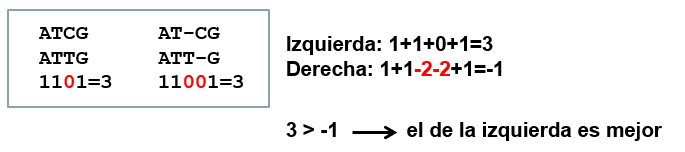
\includegraphics[width=0.5\linewidth]{figs/mejor-alineamiento.png}
\caption{Ejemplo de cálculo del mejor alineamiento.}
\end{figure}

No tiene mucho sentido alinear las secuencias de ADN de los genes codificantes de proteínas. Es mejor traducir las secuencias de ADN a secuencias de aminoácidos y alinear éstas últimas. Existen varios programas para alineamiento múltiple: clustal W/X/Omega, MAFFT, Muscle, T-Coffee, Dialign 2, etc. 

%Nos saltamos la diapositiva 42 y de la 44 a la última.


